\documentclass[border=10pt]{standalone}
\usepackage{pgfplots}
\pgfplotsset{compat=1.18, trig format plots=deg}
\begin{document}
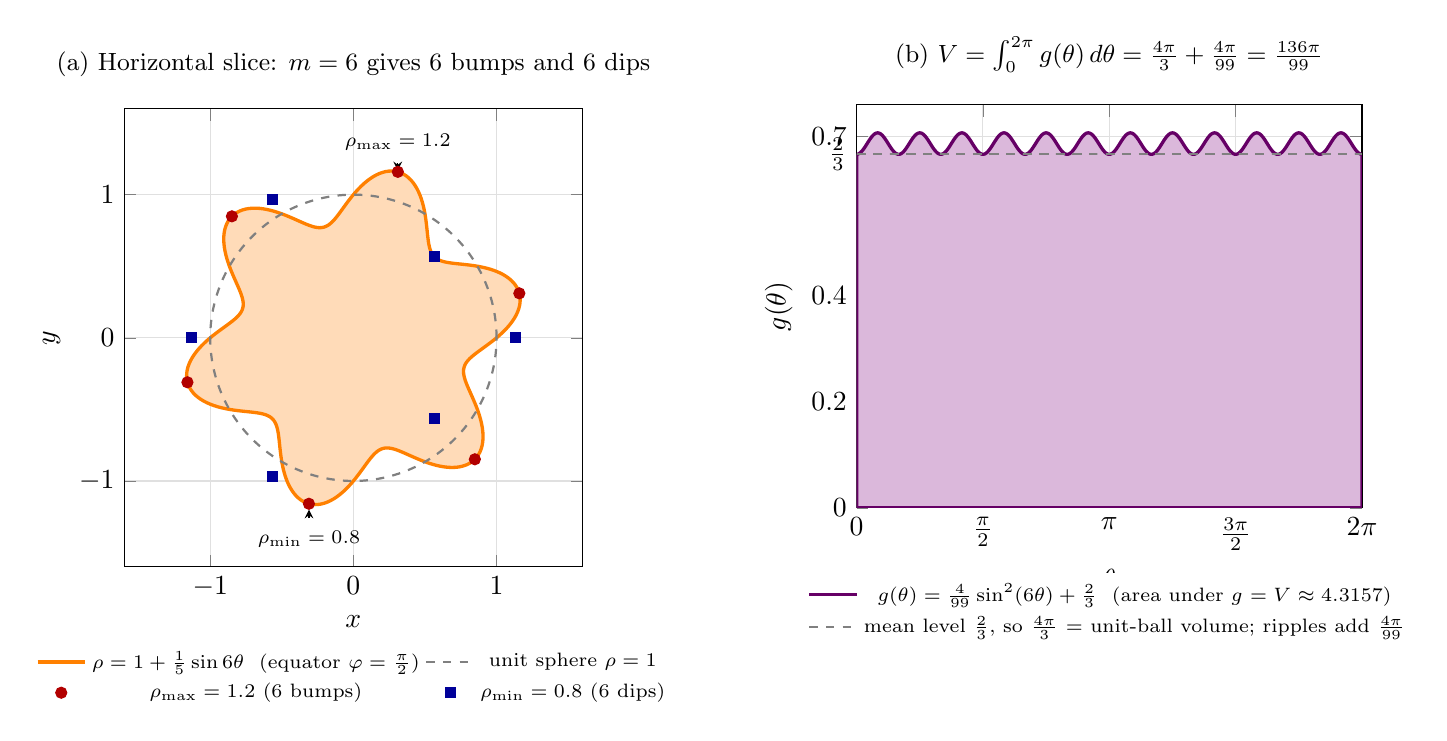
\begin{tikzpicture}

% ---------- (a) equatorial slice ----------
\begin{axis}[
    width=7.4cm, height=7.4cm,
    axis equal image,
    xmin=-1.6, xmax=1.6, ymin=-1.6, ymax=1.6,
    xtick={-1,0,1}, ytick={-1,0,1},
    xlabel=$x$, ylabel=$y$, grid=major, grid style={black!12},
    title={(a) Horizontal slice: $m=6$ gives 6 bumps and 6 dips},
    title style={align=center, yshift=2pt, font=\small},
    legend style={at={(0.5,-0.16)}, anchor=north, legend columns=2, font=\scriptsize, draw=none},
]
\addplot[domain=0:360, samples=361, very thick, orange, fill=orange!28]
  ({(1+0.2*sin(6*x))*cos(x)}, {(1+0.2*sin(6*x))*sin(x)}) \closedcycle;
\addlegendentry{$\rho=1+\frac{1}{5}\sin 6\theta$ \ (equator $\varphi=\frac{\pi}{2}$)}
\addplot[domain=0:360, samples=241, dashed, thick, gray] ({cos(x)},{sin(x)});
\addlegendentry{unit sphere $\rho=1$}
\addplot[only marks, mark=*, mark size=2.0pt, black, red!70!black] coordinates
  {(1.1591,0.3106) (0.3106,1.1591) (-0.8485,0.8485) (-1.1591,-0.3106) (-0.3106,-1.1591) (0.8485,-0.8485)};
\addlegendentry{$\rho_{\max}=1.2$ (6 bumps)}
\addplot[only marks, mark=square*, mark size=1.8pt, black, blue!60!black] coordinates
  {(0.5657,0.5657) (-0.5657,0.9659) (-1.1314,0) (-0.5657,-0.9659) (0.5657,-0.5657) (1.1314,0)};
\addlegendentry{$\rho_{\min}=0.8$ (6 dips)}
\node[font=\scriptsize, anchor=south, text=black] at (axis cs:0.31,1.24) {$\rho_{\max}=1.2$};
\draw[-stealth, thin] (axis cs:0.31,1.22) -- (axis cs:0.31,1.17);
\node[font=\scriptsize, anchor=north, text=black] at (axis cs:-0.31,-1.28) {$\rho_{\min}=0.8$};
\draw[-stealth, thin] (axis cs:-0.31,-1.26) -- (axis cs:-0.31,-1.20);
\end{axis}

% ---------- (b) reduced integrand, area under g = V ----------
\begin{axis}[
    at={(9.3cm, 0.75cm)}, anchor=south west,
    width=8.0cm, height=6.7cm,
    domain=0:360, samples=1441,
    xmin=0, xmax=360, ymin=0, ymax=0.760,
    xtick={0,90,180,270,360},
    xticklabels={$0$, $\frac{\pi}{2}$, $\pi$, $\frac{3\pi}{2}$, $2\pi$},
    ytick={0,0.2,0.4,0.6667,0.7},
    yticklabels={$0$, $0.2$, $0.4$, $\frac{2}{3}$, $0.7$},
    xlabel=$\theta$, ylabel=$g(\theta)$,
    grid=major, grid style={black!12},
    title={(b) $V=\int_0^{2\pi} g(\theta)\,d\theta=\frac{4\pi}{3}+\frac{4\pi}{99}=\frac{136\pi}{99}$},
    title style={align=center, yshift=2pt, font=\small},
    legend style={at={(0.5,-0.16)}, anchor=north, legend columns=1, font=\scriptsize, draw=none},
]
\addplot[very thick, violet!80!black, fill=violet!28] {(4/99*sin(6*x)^2+2/3)} \closedcycle;
\addlegendentry{$g(\theta)=\frac{4}{99}\sin^{2}(6\theta)+\frac{2}{3}$
                \ (area under $g$ $=V\approx 4.3157$)}
\addplot[dashed, thick, gray] {2/3};
\addlegendentry{mean level $\frac{2}{3}$, so $\frac{4\pi}{3}$ = unit-ball volume; ripples add $\frac{4\pi}{99}$}
\end{axis}

\end{tikzpicture}
\end{document}
